\chapter{Datenbeschaffung}\label{ch:data}

\section{Die ARD-Audiothek}

Die ARD Audiothek bietet ein gemeinsames Audioportal, das von den Landesrundfunkanstalten der ARD und dem Deutschlandradio betrieben wird.

Die App der Audiothek hat im Google PlayStore über eine Millionen Downloads und im Appstore [TODO]

Insgesamt hören in Deutschland ca. 

\section{Die ARD-Audiothek API}

Die Inhalte in der ARD Audiothek kann man entweder dirkt über die die Webseite erreichen, oder mithilfe einer frei benutzbare Web-GraphQL API abfragen.
(https://api.ardaudiothek.de/graphql) 
Über diese Schnittstelle bekommt man alle Informationen, wie den Titel, die Beschreibungen, die Autoren und auch den Link zu dem mp3 file jeder Episode.

Über die Abfrage \autoref{app:supplemental-information} erhält man alle Podcast Episoden des Podcasts "Radio Wissen" von bayern2.
Das sind (Stand 3. Januar 24) 2257 Podcast Episoden.
Dabei kommt es insgesamt 15 mal vor, dass zwei Episoden den selben Titel tragen, aber eine unterschiedliche Download-URL aufweisen.
Die URL unterscheidet sich nur, indem hinten die Zeichen "-1" oder "-2" angefügt wurden.
Zum Beispiel hat die Episode "Quantenphysik - Wahr, aber verrückt" den Downloadlink https://media.neuland.br.de/file/1804047/c/feed/quantenphysik-wahr-aber-verrueckt.mp3 aber auch https://media.neuland.br.de/file/2069613/c/feed/quantenphysik-wahr-aber-verrueckt-1.mp3.
In diesem Fall liefert nur die zweite URL einen Download, die erste zeigt eine Fehlermeldung an.
Es gibt auch Fälle in denen beide Links funktionieren, wie zum Beispiel 
https://media.neuland.br.de/file/32891/c/feed/die-bamberger-hexenprozesse-unschuldig-muss-ich-sterben.mp3 und
https://media.neuland.br.de/file/1858845/c/feed/die-bamberger-hexenprozesse-unschuldig-muss-ich-sterben-1.mp3   

Eine Vermutung für die doppelte Verfügbarkeit der Episoden gibt es nicht. TODO

Jede dieser Episoden ist ungefähr 20 Minuten lang und verbraucht ungefähr 20 MB Speicherplatz.
Zusammen sind diese Audiodaten ungefähr 47 GB groß.

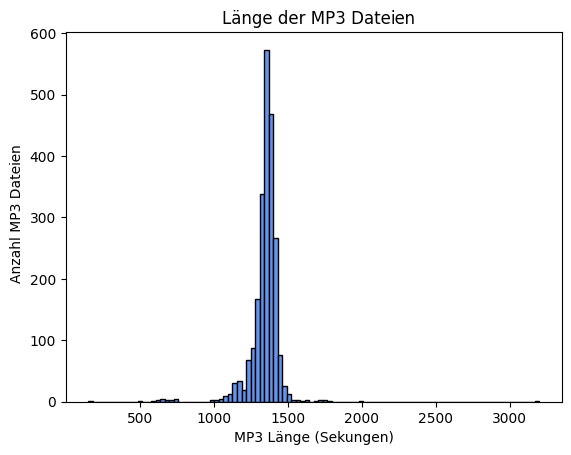
\includegraphics[width=\linewidth]{figures/mp3_length.png}

Die Transkripte der Episoden sind meißt ca. 3000 Wörter lang und benötigen ungefähr 20 KB Speicherplatz. [TODO Graphiken einfügen]







Über die API kann auch in einigen Fällen direkt ein Transkript des Audiofiles angefordert werden. 
Allerdings ist die Transkription meist nicht sehr akkurat.


Zum Beispiel steht in der Transkription des Satzes ... TODO
Das liegt daran, das die Transkriptionen mithilfe der Tools vom Fraunhofer Instituts erstellt werden, welches vermutlich veraltete Technik benutzt.


